\subsubsection{UI Komponenten}
\label{ssub:ui_komponenten}

  In diesem Abschnitt sollen die verschiedenen UI-Komponenten vorgestellt werden.

  \subsubsection*{Die Karte}
  \label{ssub:die_karte}
    Die Karte (\ref{fig:map}) ist standardmäßig auf den Längengrad 9.244 und Breitengrad 48.757 ausgerichtet. Damit findet sich der Anwender beim Aufrufen der Applikation gleich an der richtigen Stelle wieder. Die Karte verwendet eine abgeänderte Version des Kartenstils \texttt{Mapbox-Dark}. Dabei wurden Parks, Grünflächen und Wasser subtil eingefärbt und die Routen des GTFS-Feeds mit einem leichtem Orange hervorgehoben.

    \begin{figure}[htbp]
      \begin{center}
        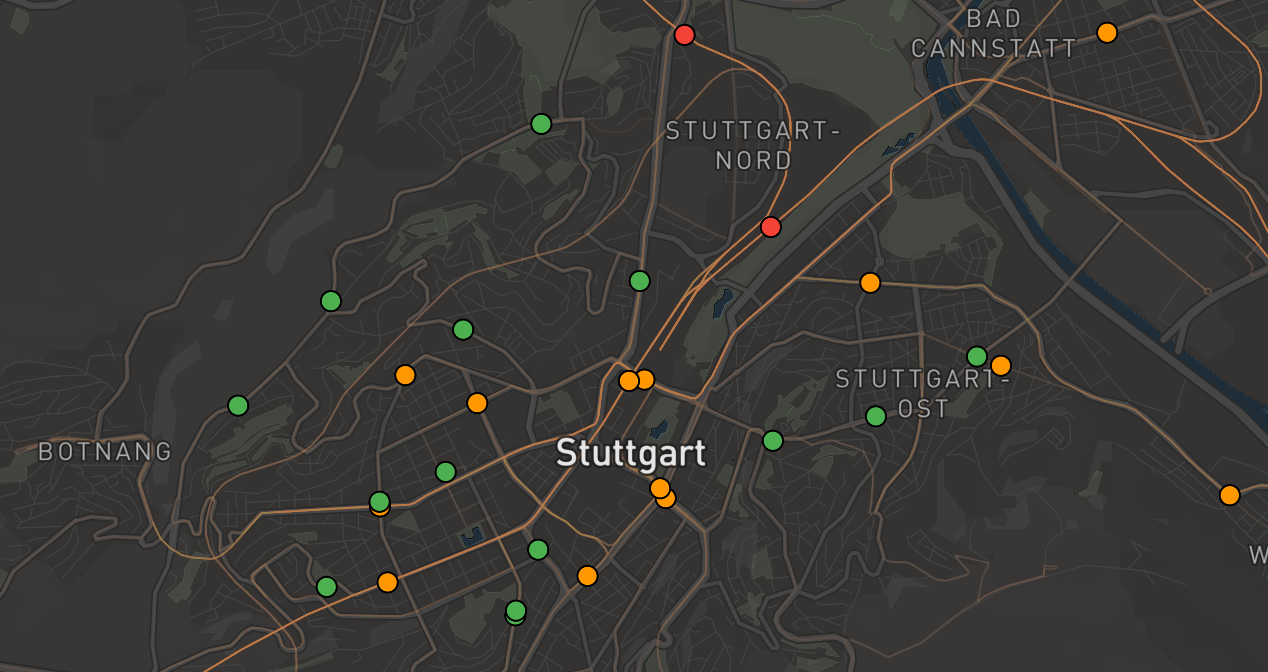
\includegraphics[width=0.6\textwidth]{map}
        \caption{Die Karte mit angepasstem Style: Mapbox-Dark}
        \label{fig:map}
      \end{center}
    \end{figure}
    
  % subsubsection die_karte (end)

  \subsubsection*{Vehicle}
  \label{ssub:vehicle_auf_karte}
    Die Vehicle sind auf der Karte als Kreis dargestellt. Die gegebene Farbe orientiert sich dabei an den öffentlichen Farben des Verkehrsunternehmens. Zum Beispiel sind Interrail Züge im Rot der Deutschen Bahn dargestellt und die U und S-Bahn hat das Orange von Stuttgart-VVS.\\

    Vehicle werden auf der Karte Animiert, wenn sie aktiv. Abbildung \ref{fig:vehicle_states} zeigt die zwei verschiedenen Animationen, die ein Vehicle beim Beginnen und Beendigen des Trips annehmen kann. Wird ein Trip aktiv, so wird das dazugehörende Vehicle auf die Karte platziert. Dabei ist der Radius des Vehicles verringert, bis er der Größe der anderen Vehicle entspricht.

    \begin{figure}[htbp]
      \centering
      \subfloat[Vehicle beginnt seinen Trip und wird aktiv]{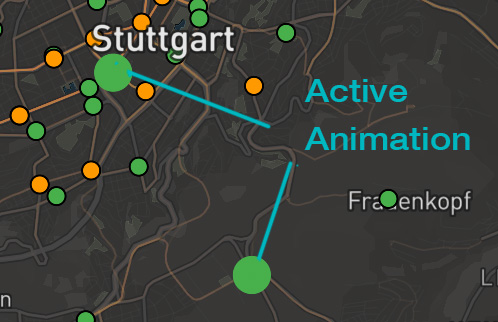
\includegraphics[width=0.34\textwidth]{vehicle_active.jpg}\label{fig:vehicle_active}}
      \hfill
      \subfloat[Vehicle beendet seinen Trip innerhalb von 30 Sekunden und wird inaktiv]{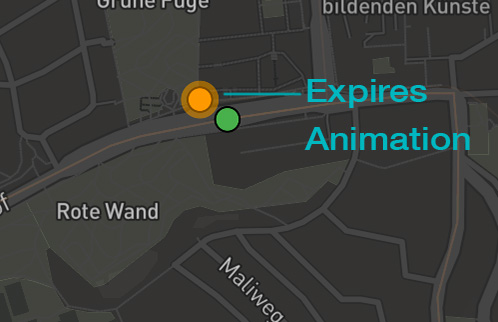
\includegraphics[width=0.34\textwidth]{vehicle_expires.jpg}\label{fig:vehicle_expires}}
      \caption{Vehicle Status Anzeige}
      \label{fig:vehicle_states}
    \end{figure}

    
    Ist ein Vehicle dabei seinen Trip innerhalb von 30 Sekunden zu beenden, so wird ein leicht transparentes Pulsieren angezeigt. Nachdem das Vehicle den Trip beendet hat, wird es von der Karte genommen und verschwindet. Technisch betrachtet werden erst alle Referenzen auf das Vehicle beseitigt und anschließend das Vehicle Objekt gelöscht.
    
  % subsubsection vehicle (end)

  \subsubsection*{Zeitstrahl}
  \label{ssub:zeitstrahl}
    Der Zeitstrahl in Abbildung \ref{fig:timeline} besteht aus mehreren Einzelteilen. 

    \begin{figure}[htbp]
      \begin{center}
        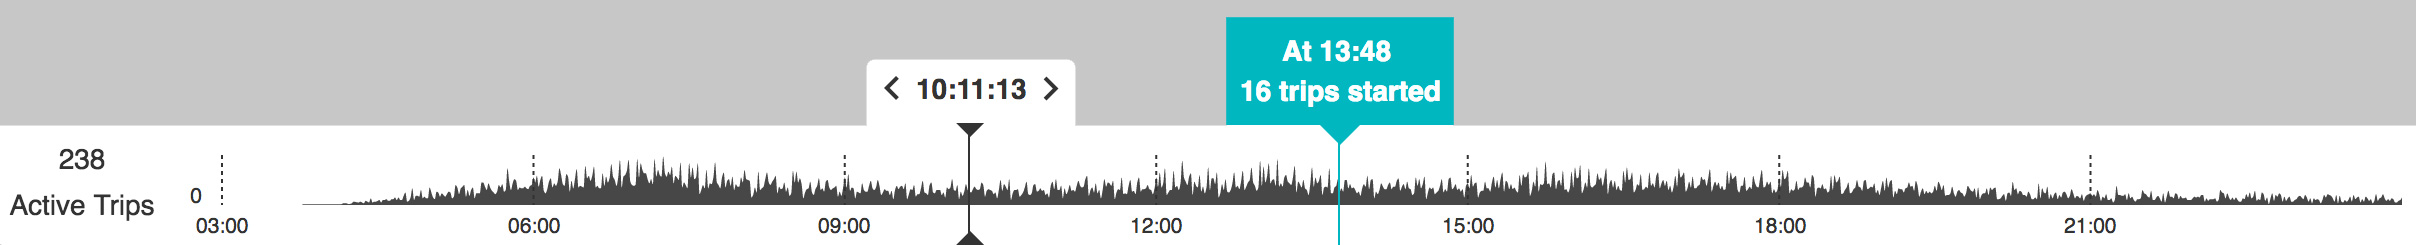
\includegraphics[width=\textwidth]{timeline}
        \caption{Zeitstrahl Komponente}
        \label{fig:timeline}
      \end{center}
    \end{figure}

    Links unten ist die Anzahl an momentan aktiven Trips zu sehen. Diese Anzahl korreliert mit den Vehicles auf der Karte. Die Anzeige wird immer aktuell gehalten und steigt, falls neue Trips aktiv werden, oder fällt wenn ein Trip beendet ist. Der Zeitstrahl selbst zeigt die Anzahl an aktiv werdenden Trips pro Minute an. Bewegt der Anwender die Maus darüber, so bekommt er die genaue Trip Anzahl zu einer Uhrzeit als Tooltip angezeigt. Ebenfalls ist es möglich die Animation zu einem beliebigem Zeitpunkt anzuzeigen. Dafür kann der Anwender einfach auf die gewünschte Zeitmarke im Zeitstrahl klicken und die Animation aktualisiert sich. Damit lässt sich die Karte zu unterschiedlichen Tageszeiten untersuchen. Zuletzt ist auch die gewählte Uhrzeit auf dem Zeitstrahl zu sehen. Diese zeigt dem Anwender, welcher Zeitpunkt momentan auf der Karte angezeigt wird.
    
  % subsubsection zeitstrahl (end)

  \subsubsection*{Filter}
  \label{ssub:filter}
    Über ein ausklappbares Menü, lassen sich verschiedene Filter auswählen. Dadurch kann der Anwender zum Beispiel alle Vehicle eines Typs oder einer Linie darzustellen. Auch Kombinationen der \texttt{Filter Vehicles} und \texttt{Filter Lines} sind möglich. Da aber meist eine Linie von genau einem Vehicle Typ bedient wird, macht das oft keinen Sinn.

    Damit der Anwender die Relation zwischen dem Filter und den Vehicle auf der Karte versteht, sind die Farben einheitlich gestaltet. Nachdem ein Filter ausgewählt ist, kann das Menü entweder wieder zugeklappt werden, oder der Filter lässt sich wieder abwählen.

    \begin{figure}[htbp]
      \begin{center}
        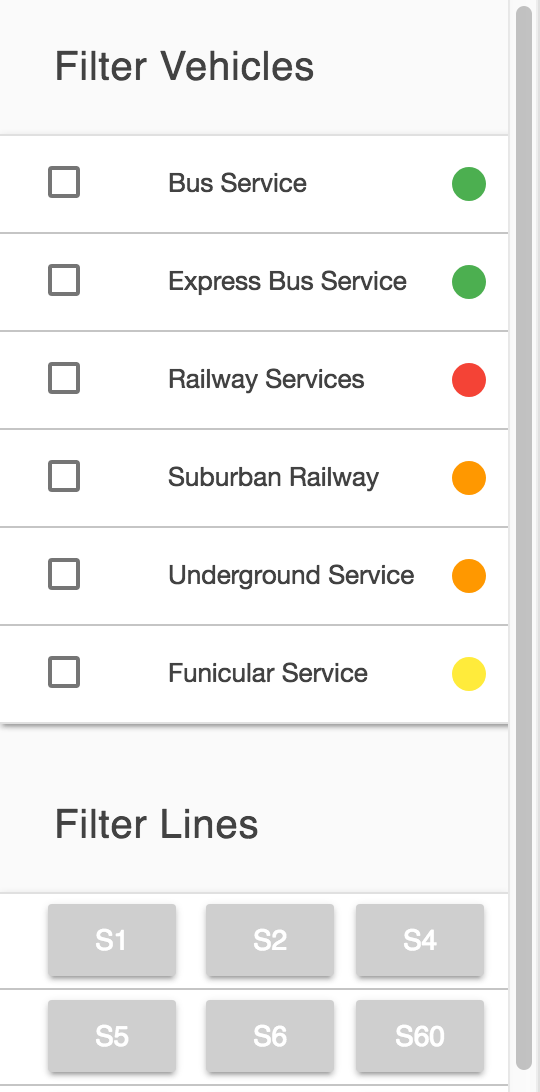
\includegraphics[width=0.2\textwidth]{filter}
        \caption{Filter Funktion}
        \label{fig:filter}
      \end{center}
    \end{figure}
    
  % subsubsection filter (end)

  \subsubsection*{Anzeigen von Trip Informationen}
  \label{ssub:anzeigen_von_trip_informationen}
    Wenn der Anwender ein Vehicle in der Karte durch Klicken auswählt, öffnet sich ein Fenster, welches Informationen für diesen Trip anzeigt (Abbildung \ref{fig:trip_information}. Neben dem Namen der Route lässt sich im Kreis (hier in Rot) die Routen Nummer ablesen. Im unteren Bereich sind die Fahrplaninformationen für den Trip gelistet. Neben dem Namen der Station ist auch die Abfahrtzeit des Vehicles gelistet. Die bereits besuchten Stationen werden in einem Grauton dargestellt um sie als inaktiv zu markieren.


    \begin{figure}[htbp]
      \begin{center}
        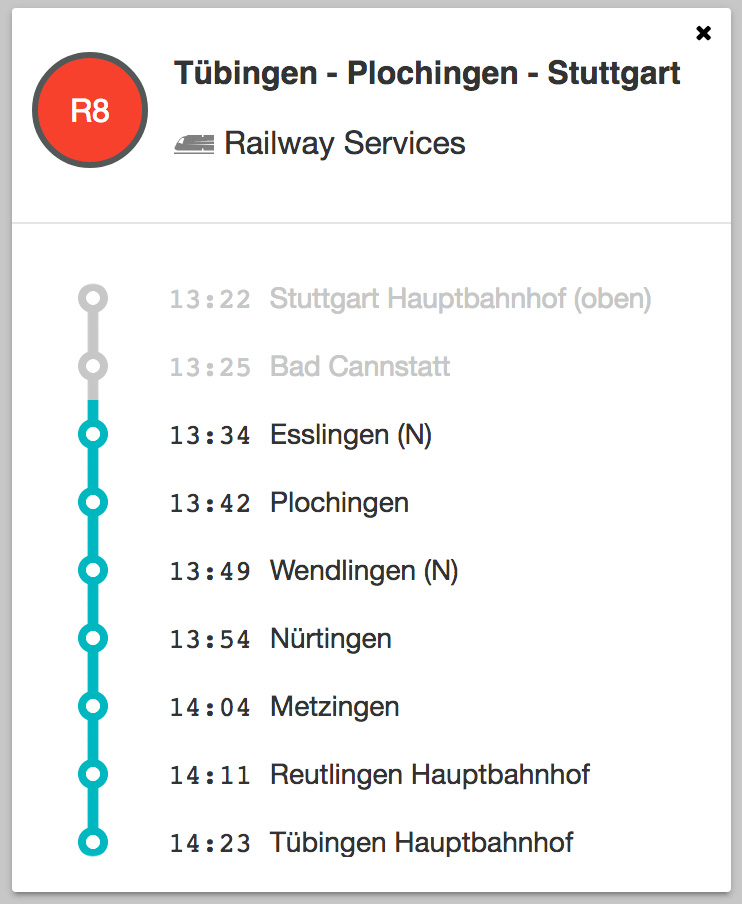
\includegraphics[width=0.3\textwidth]{trip_information}
        \caption{Anzeigen von Trip Informationen}
        \label{fig:trip_information}
      \end{center}
    \end{figure}

    \pagebreak
    
  % subsubsection anzeigen_von_trip_informationen (end)

  \subsubsection*{Wechseln der Kartendarstellung}
  \label{ssub:style_auswahl}
    Über das \texttt{Switch Style} \inlinegraphics{switch_styles_symbol} Element hat der Anwender die Möglichkeit zwischen verschiedenen Darstellungsarten der Karte zu wechseln. Auch die Polylines der Routen lassen sich zusätzlich über das Anwählen von \texttt{Shape} ein- oder ausblenden. Standardmäßig ist \texttt{Dark} ausgewählt.

    \begin{figure}[htbp]
      \begin{center}
        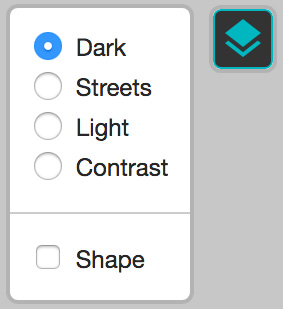
\includegraphics[width=0.14\textwidth]{switch_styles}
        \caption{Wechseln zwischen verschiedenen Kartendarstellung}
        \label{fig:switch_styles}
      \end{center}
    \end{figure}
    
  % subsubsection style_auswahl (end)

  \subsubsection*{Linien Finder}
  \label{ssub:linien_finder}
    Durch klicken des \texttt{Line Finder} \inlinegraphics{line_finder_symbol} Buttons lässt sich auf der Karte eine Route finden, die zwei Stationen $A, B$ verbindet. Dafür setzt der Anwender zwei Pins auf die Karte. Danach sucht ein Algorithmus diejenige Route aus, die am besten diese Stationen verbindet. Das Ergebnis sieht dann wie folgt aus:

    \begin{figure}[htbp]
      \begin{center}
        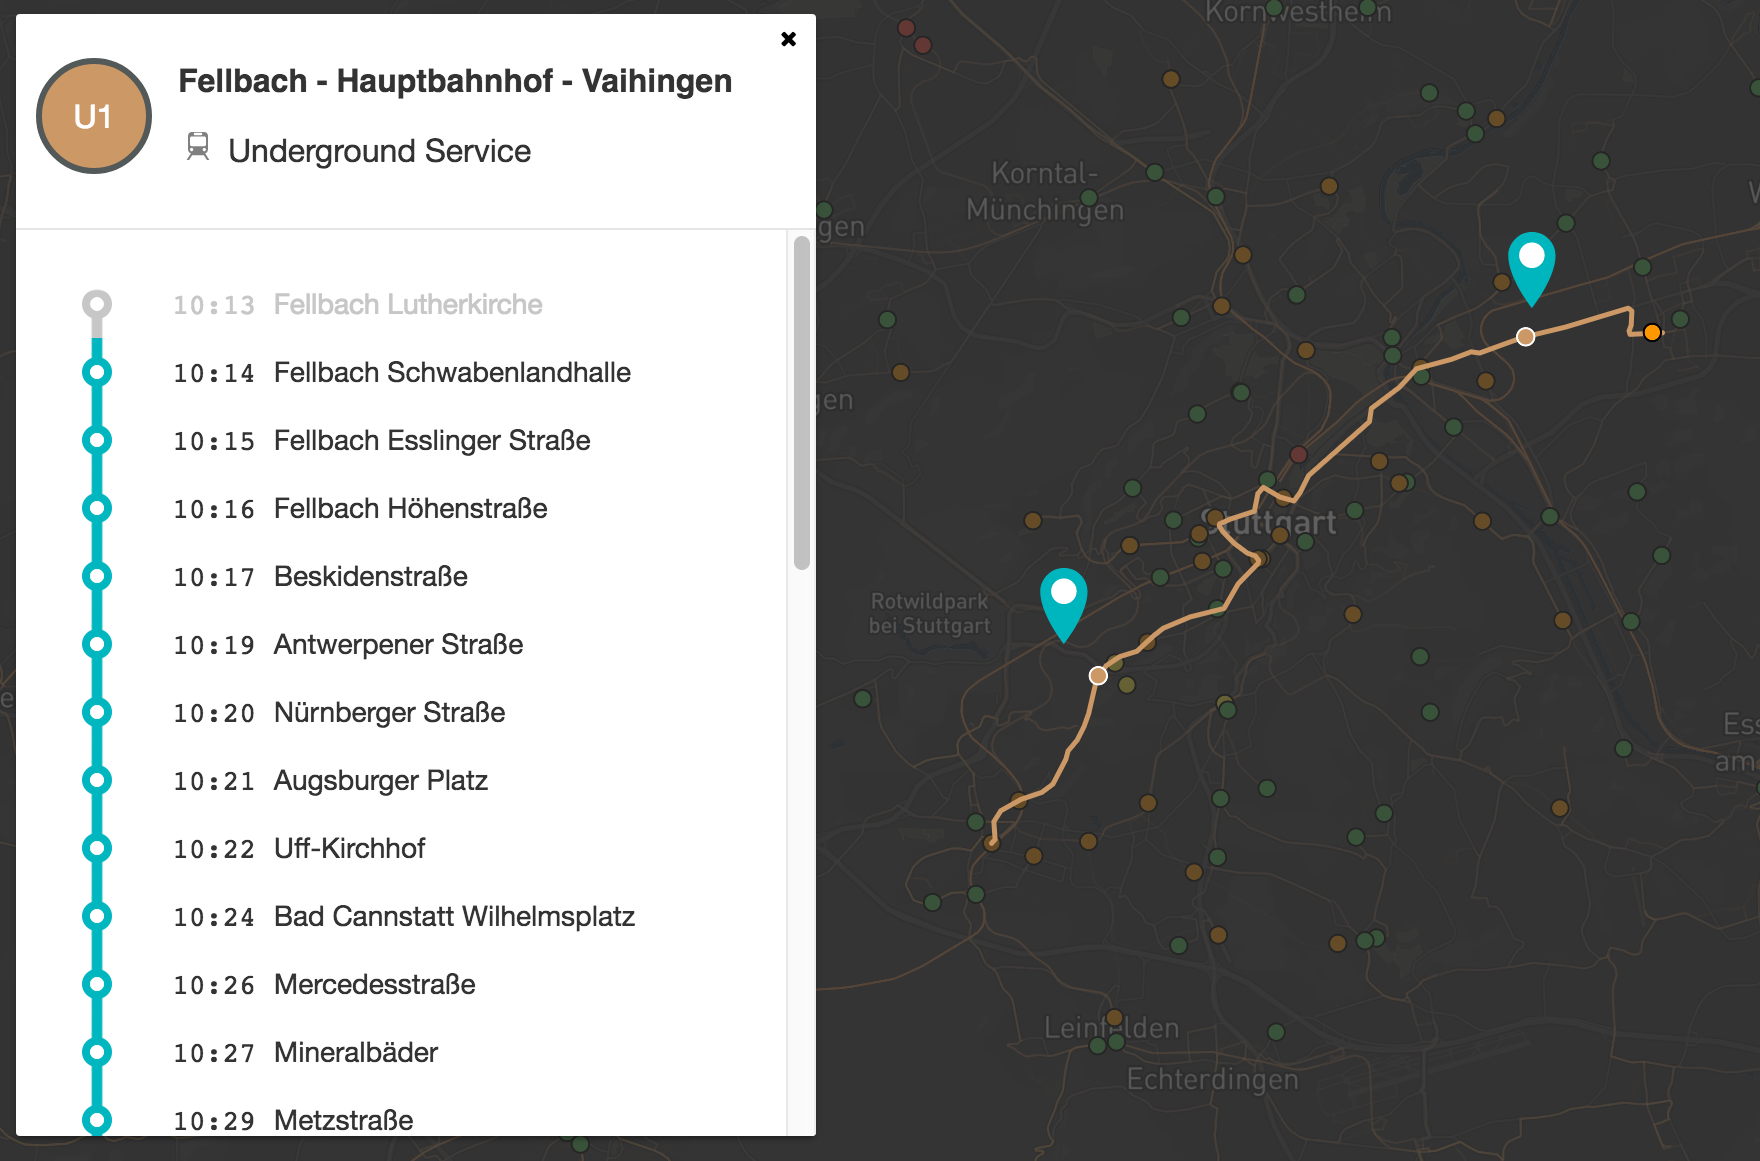
\includegraphics[width=0.6\textwidth]{line_finder}
        \caption{Linien Finder}
        \label{fig:line_finder}
      \end{center}
    \end{figure}

    Diese Funktion vereint Visualisierung und Wegfindung in einer Applikation. Während wir momentan ausschließlich eine Wegfindung über verschiedene Formularfelder (Von..., Nach..., Datum, Uhrzeit) beginnen, könnte es für städtische oder regionale Wegfindung auch eine visuelle Lösung geben. Der Vorteil liegt dabei, dass kein Kontextwechsel nötig ist. Die Orientierung, Wegfindung und Fahrplaninformationen ließen sich alle in einer Ansicht unterbringen. Ein weiteres Merkmal dieses visuellen Ansatzes ist die Möglichkeit eine Route zu finden, ohne dass die Namen der Haltestellen bekannt sein müssen. Das auf der Karte dargestellte Ergebnis, zeigt dem Nutzer auch gleich, wo sich das zur Route gehörende Vehicle sich befindet. Damit könnte der Anwender auch gleich entscheiden, ob er dieses Vehicle noch erreichen würde oder nicht. Dabei ließen sich auch sehr gut GTFS-Realtime Informationen verwenden, so dass man gleich sehen würde ob das Vehicle zum Beispiel Verspätung hat.\\

    Von allen implementierten Komponente hat der Linien Finder am meisten Potential für verschiedene Weiterentwicklungen. Angefangen von der Implementierung von Echtzeitinformationen, über eine integrierte Anwender Navigation (zum Beispiel könnte man den Anwender zu einer Station navigieren), als auch das Anbieten von Möglichkeiten zum Verbindungsanschluss wären möglich. Ebenfalls kann der Algorithmus zur Auswahl der empfohlenen Route noch sehr viel weiter verbessert werden. Momentan fließt vor allem die mittlere Distanz zwischen gesetztem Pin und nächster Station in die Entscheidung ein. Weitere Faktoren könnten aber noch berücksichtigt werden. Beispielsweise der Typ des Vehicles (U-Bahn bevorzugt gegenüber Bus), Frequenz der Route, Wartezeit auf das Vehicle, Preis, Reisezeit oder gar das momentane Verkehrsaufkommen.
    
  % subsubsection linien_finder (end)
  

  % * Timeline Component (Time jump + Trip counter, Trips that get active)
  % * Vehicles, Vehicle States (active, inactive)
  % * Filtering mechanism (Lines / Type)
  % * Layer switcher
  % * Route finder
  % * Bezier Easing 
  
% subsubsection ui_komponenten (end)
